\begin{hcarentry}{Haskino}
\label{Haskino}
\report{Mark Grebe}%10/15
\participants{Andrew Gill}
\status{active}
\makeheader

%**<img width=400 src="./jh2.jpg">
%*ignore
\begin{center}
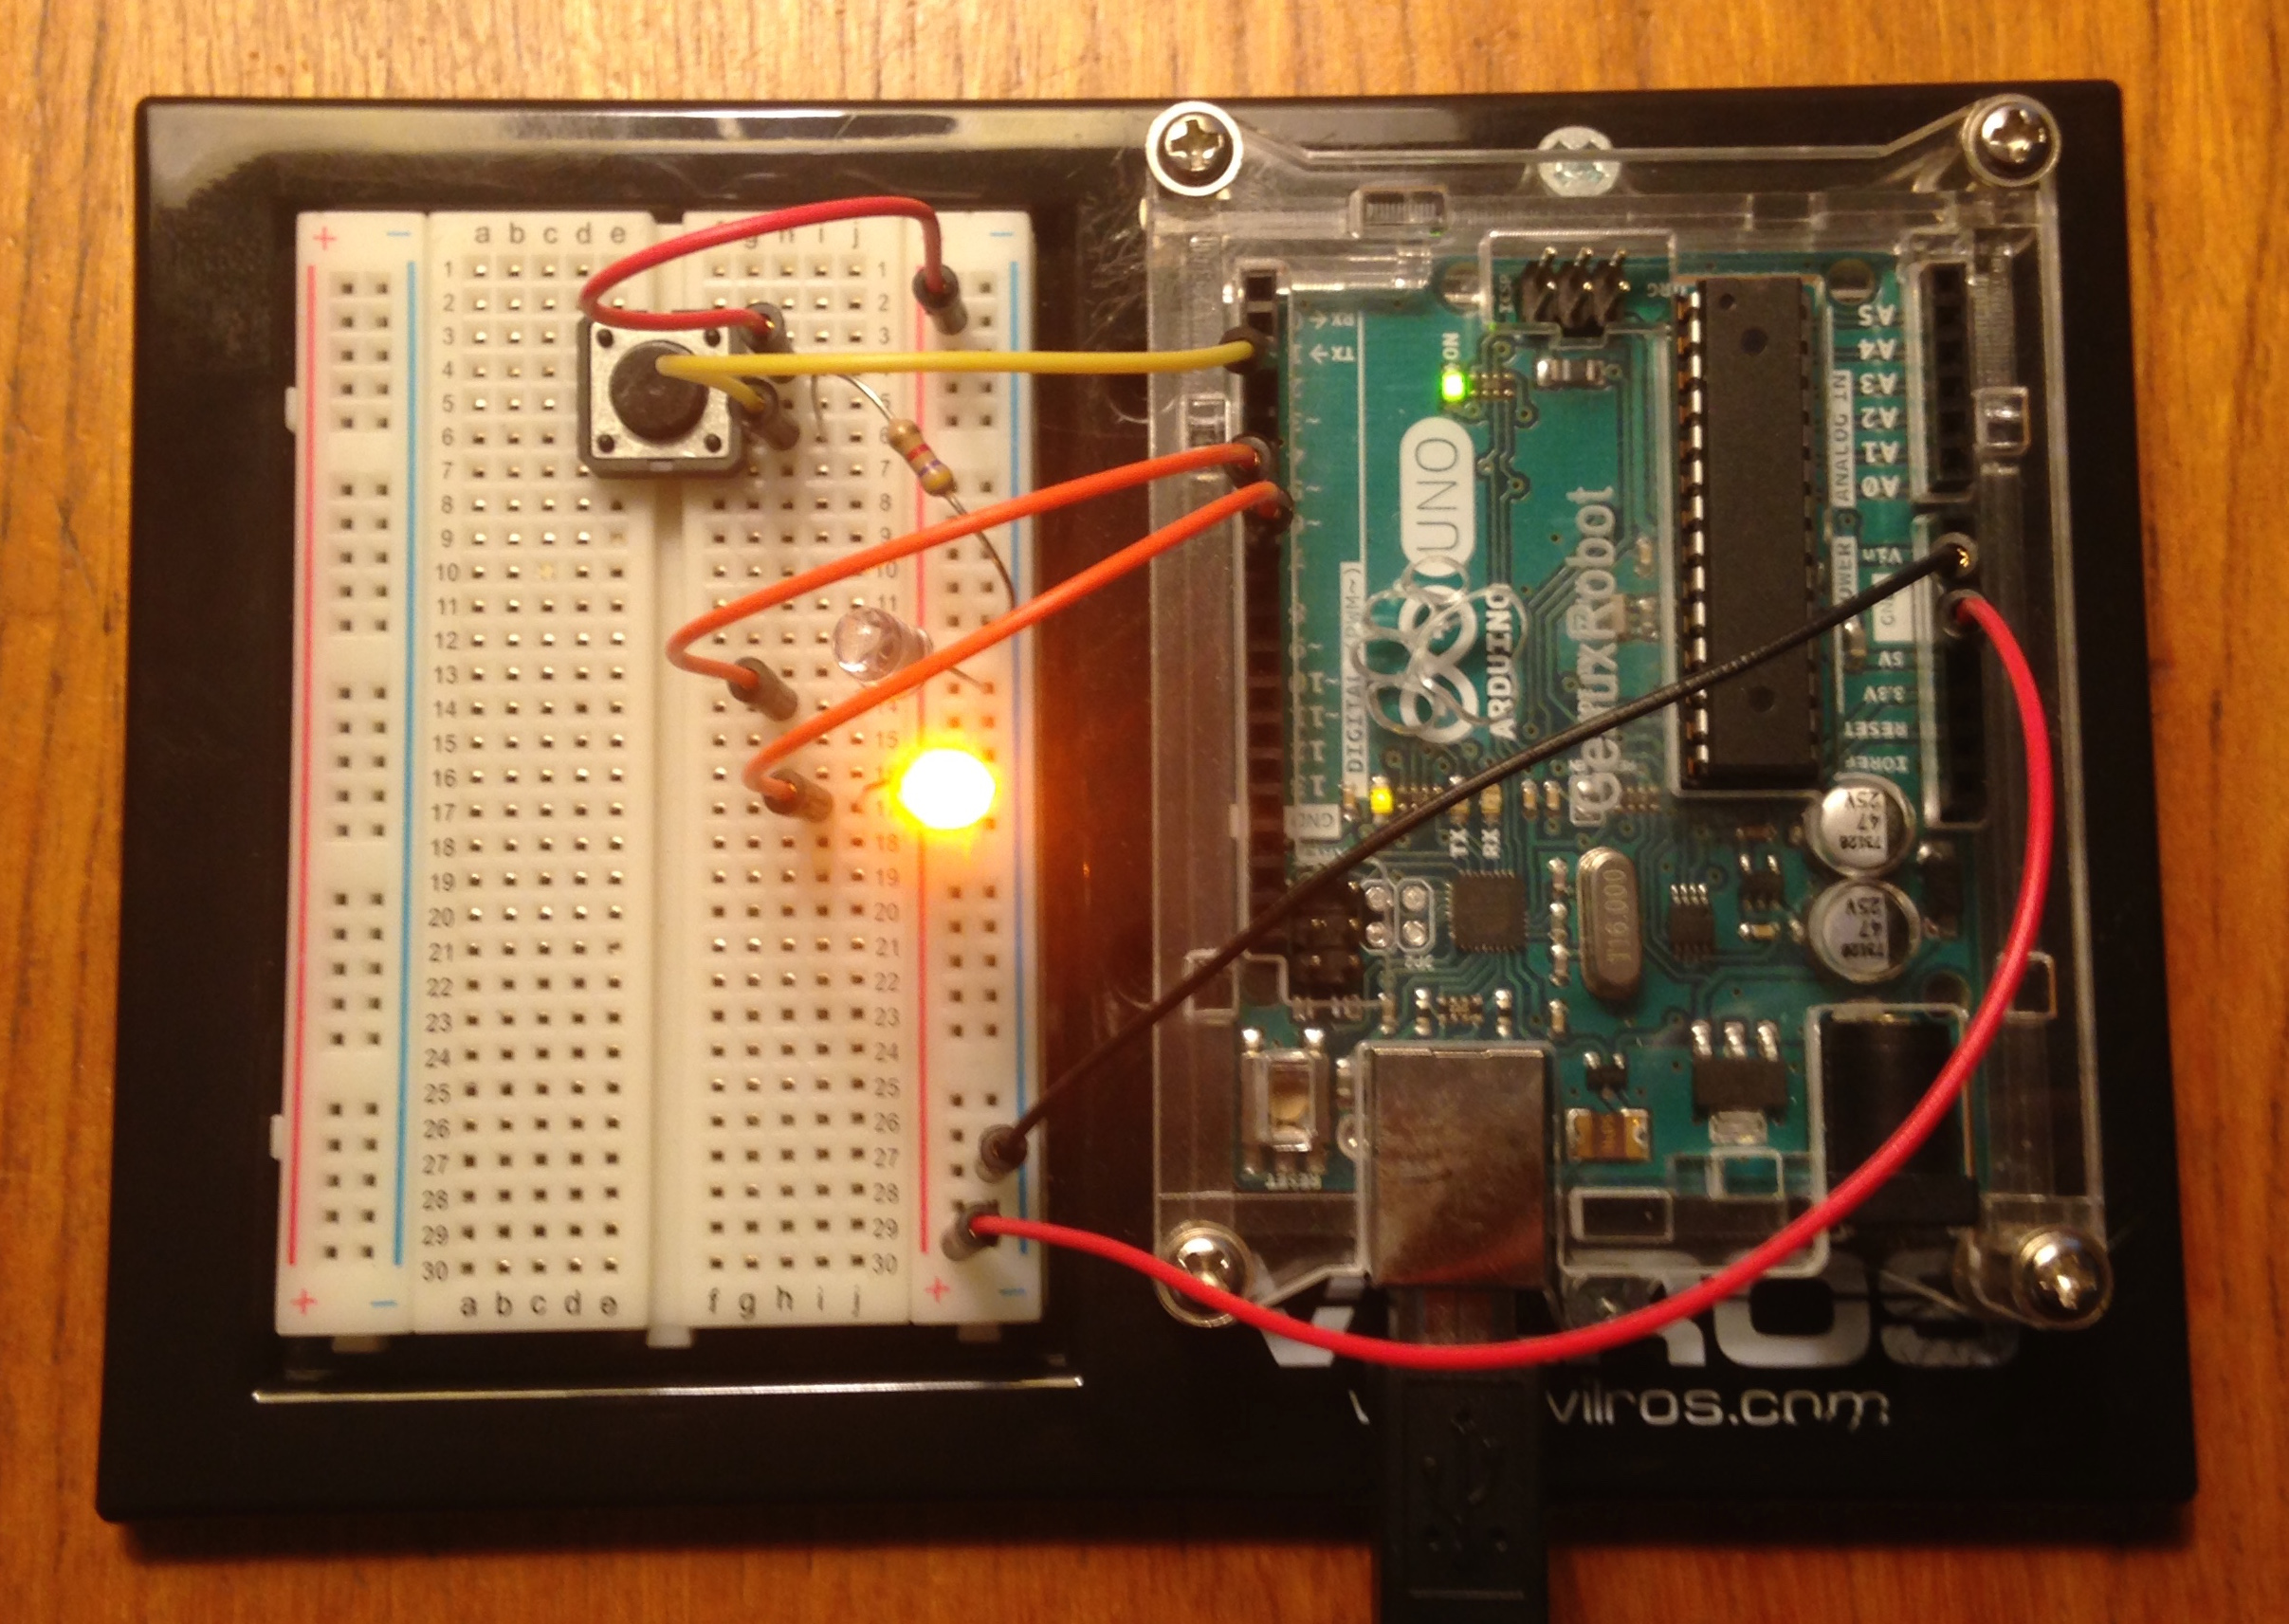
\includegraphics[width=0.435\textwidth]{html/Arduino.jpg}
\end{center}
%*endignore


Haskino is a Haskell development environment for programming the
Arduino microcontroller boards in a high level functional language
instead of the low level C language normally used.  

This work started with Levent Erk\"{o}k's hArduino package.  The original 
version of Haskino, extended hArduino by applying the concepts of the 
strong remote monad design pattern to provide a more efficient way 
of communicating, and generalizing the controls over the remote execution. 
In addition, it added a deep embedding, control structures, an expression
language, and a redesigned firmware interpreter to enable standalone 
software for the Arduino to be developed using the full power of Haskell.

The current version of Haskino continues to build on this work.
Haskino is now able to directly generate C programs from our Arduino
Monad.  This allows the same monadic program to be quickly developed
and prototyped with the interpreter, then compiled to C for more
efficient operation.  In addition, we have added scheduling capability
with lightweight threads and semaphores for inter-thread synchronization.

The development has been active over the past year.  A paper was 
published at PADL 2016 for original version, and there is a
paper accepted for presentation at TFP 2016 for the new
scheduled and compiled version.

\FurtherReading
\begin{compactitem}
\item
  \url{https://github.com/ku-fpg/haskino}
\item
  \url{https://github.com/ku-fpg/wiki}
\end{compactitem}
\end{hcarentry}
